\documentclass{article}
\usepackage[utf8]{inputenc}
\usepackage{amsmath}
\usepackage{amssymb}
\usepackage{graphicx}

\newcommand\xn{x^{\left(n\right)}}
\newcommand\xkn{x^{\left(n+1\right)}}
\newcommand\xz{x^{\left(0\right)}}
\newcommand\xstar{x^{*}}
\begin{document}
\section*{A derivative-free iterative scheme for finding zeros}
Let $f : \left[a,b\right] \mapsto \mathbb{R}$ be twice continuously differentiable with $f\left(\xstar\right) = 0$ and $f'\left(\xstar\right) \neq 0$. Consider the iteration (Steffensen's method) defined by
\begin{equation*}
    \xkn = \xn - \frac{f\left(\xn\right)}{g\left(\xn\right)} \,, \: \text{where } g\left(x\right) = \frac{f\left(x + f\left(x\right)\right) - f\left(x\right)}{f\left(x\right)}
\end{equation*}
\subsection*{8-4.a}
We are tasked with implementing the Steffensen's method. The function supplies us with a functor \verb|f| that describes the function $f$ and an inital guess \verb|x0|. We are told to terminate the iteration when the computed sequence of approximation becomes stationary. For this purpose we can check if the new approximation is the same as the current approximation up to some numerical limit, i.e.
\begin{equation*}
   \left\lvert \frac{\xn - \xkn}{\xkn}\right\rvert \leq \epsilon
\end{equation*}
where for $\epsilon$ we choose \verb|std::numeric_limits<double>::epsilon()|. This results in the following code

\begin{figure}[!hbt]
    \centering
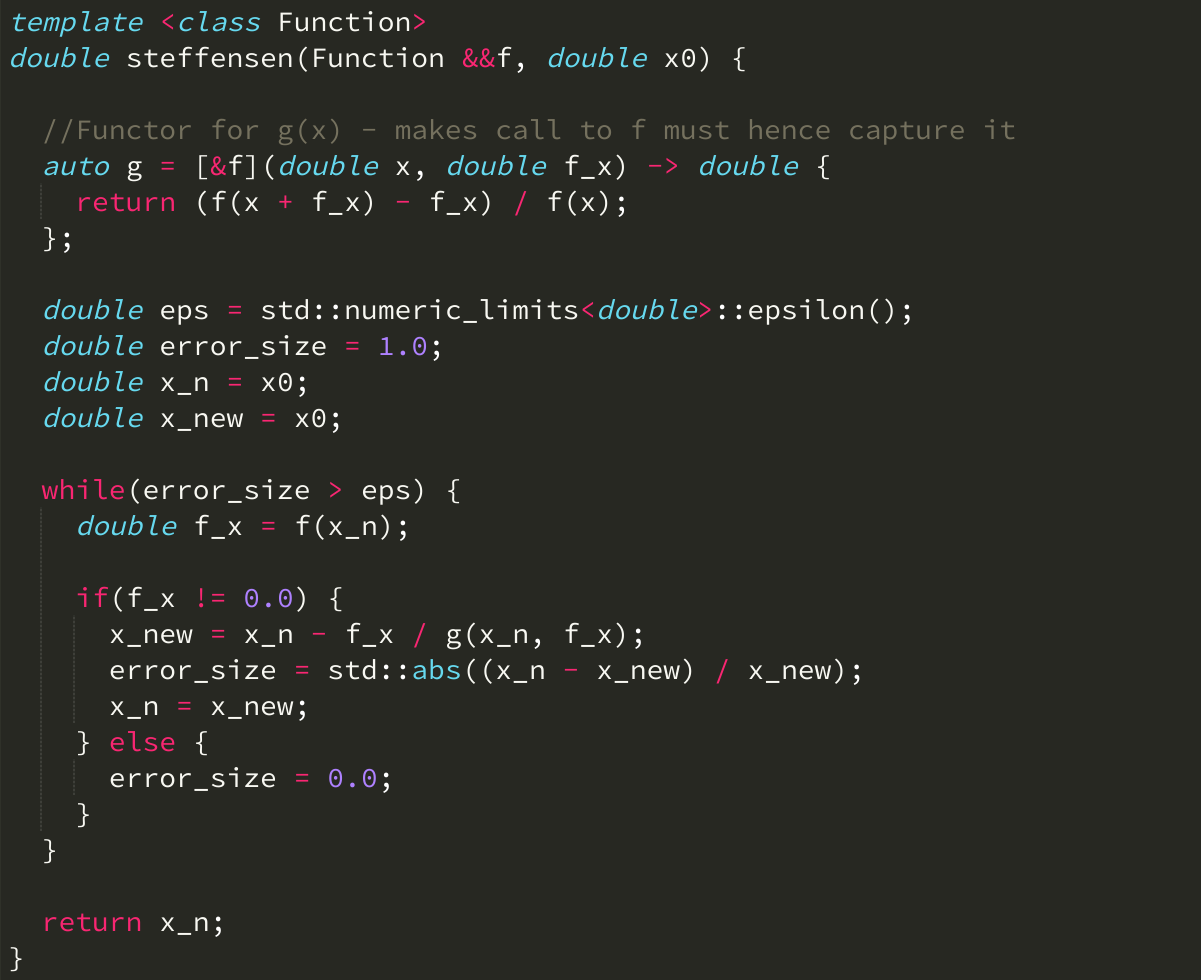
\includegraphics[width=0.9\linewidth]{8-4.a.png}
\end{figure}

\pagebreak

\subsection*{8-4.b}
We are tasked with writing a function \verb|testSteffensen| that tests our implementation to find the zero of the function
\begin{equation*}
    f\left(x\right) = xe^{x} - 1
\end{equation*}
we are told to use $\xz = 1$ as initial guess. This produces the following code.

\begin{figure}[!hbt]
    \centering
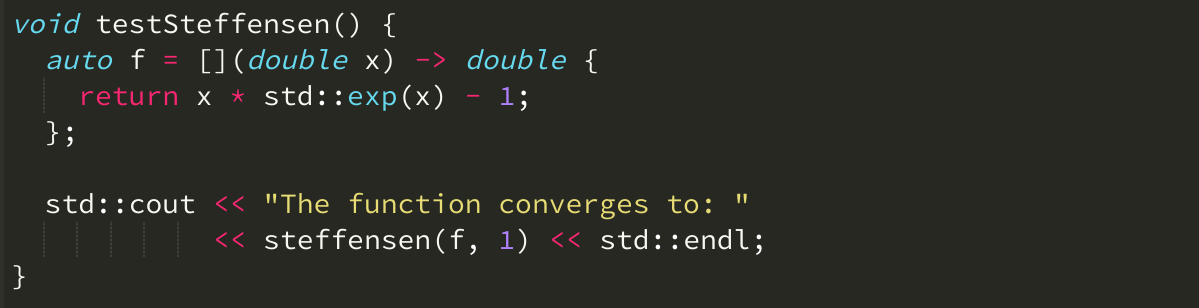
\includegraphics[width=1.0\linewidth]{8-4.b.png}
\end{figure}

\subsection*{8-4.c}
We are now tasked with extending our implementation of the Steffensen's method with a logger functor that logs each iterate. We the should use this to implement a function \verb|orderSteffensen| that tabulates values from which we can read of the order of convergence of Steffensen's method when applied to the test case of Sub-problem 8-4.b. We can test our implementation using the following two metrics, the first is the error norm of the $n$-th step
\begin{equation*}
    \epsilon_{k} := \left\lvert \xn - \xstar\right\rvert
\end{equation*}
and then for detecting convergence of order $p > 1$ we use the approximation of $p$ via
\begin{equation*}
    p \approx \frac{\log\left(\epsilon_{n+1}\right) - \log\left(\epsilon_{n}\right)}{\log\left(\epsilon_{n}\right) - \log\left(\epsilon_{n-1}\right)}
\end{equation*}
We are looking for a $\xstar$ for which
\begin{equation*}
    xe^{x} - 1 = 0
\end{equation*}
we get the solution
\begin{equation*}
    \xstar = 0.5671432904097838729999686622103555497538
\end{equation*}
we will use this value for the error computation. The order of convergence in the solution and the one recorded by my solution (and the solution shown in the master solution) do not match up, so there may be an error somewhere. 

\pagebreak

\noindent This produces the following code

\begin{figure}[!hbt]
    \centering
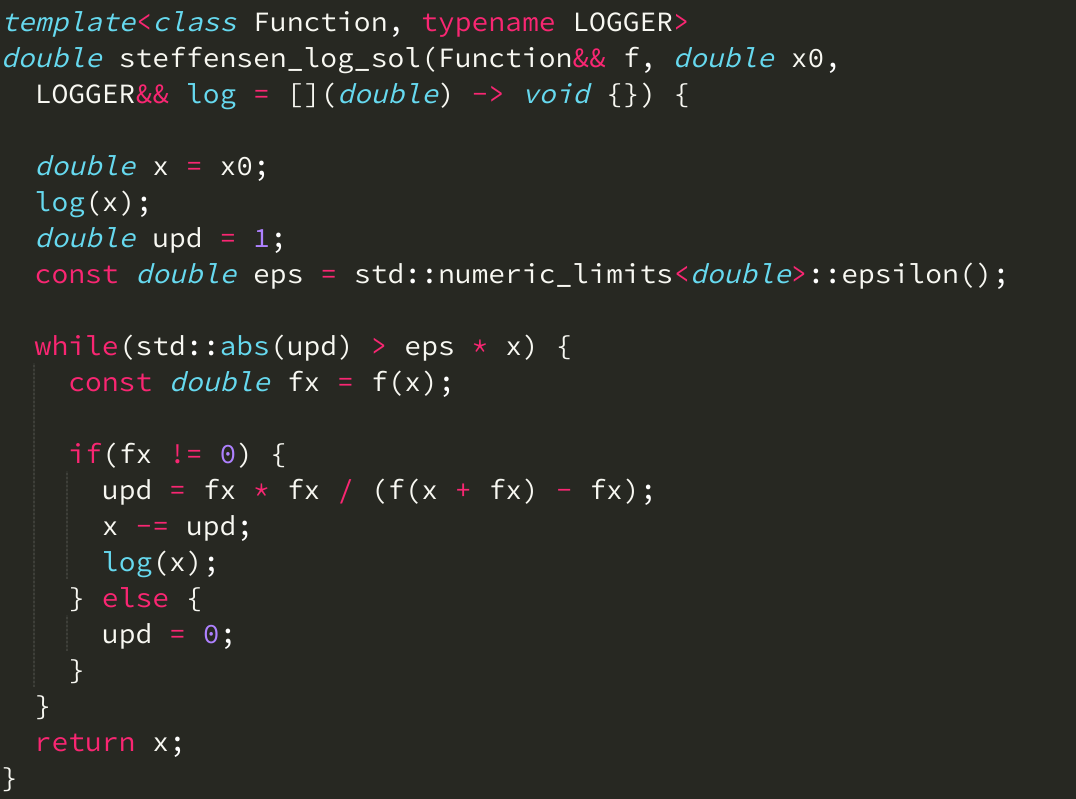
\includegraphics[width=0.7\linewidth]{8-4.c.png}
\end{figure}

\begin{figure}[!hbt]
    \centering
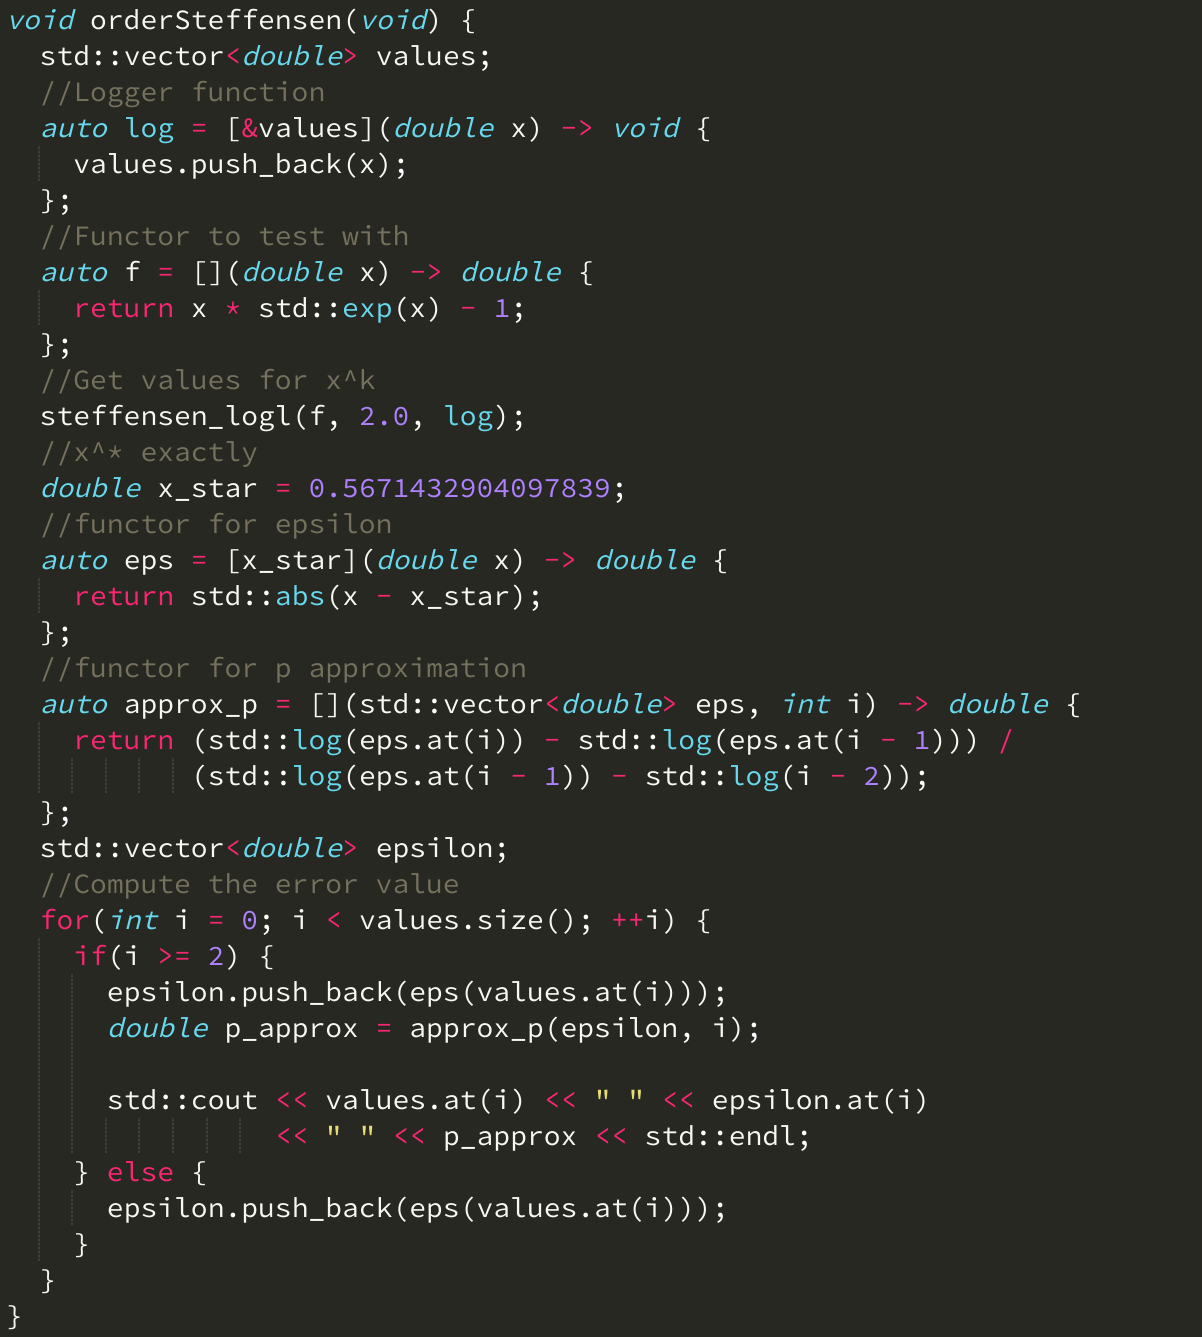
\includegraphics[width=0.7\linewidth]{8-4.c2.png}
\end{figure}

\pagebreak
\subsection*{8-4.d}
We are tasked with finding a function with the same zero as $f$ that does not involve a term $e^{xe^{x}}$ in $g$, which grows extremely fast and can thus not have a large initial guess. We can modify this by finding a function $h$ such that $h\left(x\right) \neq 0$ for all input values of $f$ and then looking for the zero of the function $\left(hf\right)\left(x\right)$. We do not take the composition of the function here but multiply them and rely on the lack of zero divisors in the real numbers. We want to eliminate the term $e^{x}$ which we can do by multiplying with $e^{-x}$, for which we have that $e^{-x}\neq 0$ for all $x\in \mathbb{R}$. We get 
\begin{equation*}
    \left(fh\right)\left(x\right) = f\left(x\right) \cdot e^{-x} =  \left(xe^{x}-1\right)e^{-x} = xe^{x}e^{-x} - e^{-x} = x -e^{-x} = \tilde{f}\left(x\right)
\end{equation*}
and for the function $g$ we get
\begin{align*}
    g\left(x\right) = \frac{\tilde{f}\left(x + x -e^{-x}\right) - x + e^{-x}}{x- e^{-x}} &= \frac{\tilde{f}\left(2x - e^{-x}\right) -x + e^{-x}}{x - e^{-x}}\\ 
    &= \frac{2x - e^{-x} - e^{-2x+e^{-x}}}{x-e^{-x}}
\end{align*}
hence $g$ does not suffer from the discussed issue anymore.

\end{document}
